\documentclass[11pt,a4paper]{article}

\usepackage[utf8]{inputenc}
\usepackage[T1]{fontenc}
\usepackage{lmodern}
\usepackage[spanish,es-tabla,es-nodecimaldot]{babel}
\usepackage[margin=2.3cm]{geometry}
\usepackage{amsmath,amssymb,mathtools}
\usepackage{booktabs}
\usepackage{array}
\usepackage{tabularx}
\usepackage{float}
\usepackage{graphicx}
\usepackage{xcolor}
\usepackage{listings}
\usepackage{tikz}
\usetikzlibrary{quantikz2,babel}
\usepackage[hidelinks]{hyperref}

% Notación de Dirac (se redefine después de cargar quantikz para evitar conflictos)
\providecommand{\ket}{}\renewcommand{\ket}[1]{\lvert #1\rangle}
\providecommand{\bra}{}\renewcommand{\bra}[1]{\langle #1\rvert}
\providecommand{\braket}{}\renewcommand{\braket}[2]{\langle #1\vert #2\rangle}
\newcommand{\ketbra}[2]{\lvert #1\rangle\!\langle #2\rvert}
\newcommand{\tfr}[2]{\tfrac{#1}{#2}}
\renewcommand{\arraystretch}{1.25}
\setlength{\emergencystretch}{3em}

\lstset{
  basicstyle=\ttfamily\small,
  columns=fullflexible,
  keepspaces=true,
  frame=single,
  rulecolor=\color{black!25},
  backgroundcolor=\color{black!3},
  commentstyle=\color{black!55}\itshape,
  keywordstyle=\color{blue!60!black}\bfseries,
  language=Python,
  literate={á}{{\'a}}1 {é}{{\'e}}1 {í}{{\'i}}1 {ó}{{\'o}}1 {ú}{{\'u}}1 {ñ}{{\~n}}1
           {→}{{$\to$}}1 {≈}{{$\approx$}}1 {π}{{$\pi$}}1 {√}{{$\surd$}}1 {·}{{$\cdot$}}1
           {⟩}{{$\rangle$}}1 {⟨}{{$\langle$}}1
}

\title{Práctica 3: Algoritmo de Grover --- Extensión para $n$ qubits\\[2pt]
\large Ejecución con 2 qubits y comparaciones}
\author{Carlos Andres Duran Paredes \quad Juan David Zapata Londoño\\[4pt]\small Universidad de Antioquia --- Computación Cuántica --- Práctica de Laboratorio No.~3}
\date{}

\begin{document}
\maketitle
\vspace{-0.6cm}

%==================================================================
\section{Introducción y objetivo}

La actividad~2 (10\,\%) de la Práctica~3~\cite{enunciado} pide analizar el notebook del curso\\
\texttt{N-Grover\_AnyMark\_2026.ipynb}~\cite{ngrover}, que extiende el algoritmo de Grover del
tutorial de IBM~\cite{ibm} a $n$ qubits y a cualquier estado marcado; ejecutar su simulación para
\textbf{2 qubits}; y comparar esa ejecución con (i) la del tutorial original de Qiskit y (ii) el
análisis manual de la actividad~1~\cite{parte1,pasoapaso}.

La ejecución se hizo con el notebook \texttt{notebooks/Actividad2\_N\_Grover\_2qubits.ipynb}. Los resultados que se
citan aquí se reprodujeron también con el notebook\\
\texttt{notebooks/Actividad2\_Comparacion\_Tutorial.ipynb}, que ejecuta
en el mismo entorno el circuito del tutorial y compara matrices y estados. Las figuras~\ref{fig:hist} y~\ref{fig:iter} se generan con
\texttt{docs/generar\_figuras\_actividad2.py}. El análisis manual de la actividad~1 lo desarrolló Juan David Zapata Londoño y se
publica por separado; aquí solo se usan sus resultados para comparar.

\paragraph{Convención.} Como en la actividad~1, se usa el orden \emph{little-endian} de Qiskit:
en $\ket{q_1q_0}$ el qubit $q_0$ es el dígito de la derecha. Para 2 qubits la base se ordena
$\ket{00},\ket{01},\ket{10},\ket{11}$, y el estado buscado es $\ket{q_1q_0}=\ket{01}$
($q_1=0$, $q_0=1$), el mismo del tutorial.

%==================================================================
\section{Análisis del notebook N-Grover}

\subsection{Qué hace cada celda}

\begin{table}[H]
\centering
\small
\begin{tabularx}{\textwidth}{@{}c>{\raggedright}p{5.2cm}>{\raggedright\arraybackslash}X@{}}
\toprule
Celda & Contenido & Función\\
\midrule
0 & \texttt{QuantumCircuit}, \texttt{Statevector}, \texttt{numpy} & Importaciones.\\
1 & \texttt{n = 3}, \texttt{MarkState = '011'} & Número de qubits y estado marcado (MSB $\to$ LSB).\\
2 & \texttt{Oracle(qc, target\_state)} & Oracle de fase para \emph{cualquier} estado marcado.\\
3 & \texttt{diffusion\_operator(circuit)} & Difusor $H^{\otimes n}(\cdots)H^{\otimes n}$ sobre los $n$ qubits.\\
4 & \texttt{grover\_circuit.h(range(n))} & Inicialización: superposición uniforme.\\
5--6 & \texttt{Oracle(...)}, \texttt{diffusion\_operator(...)} & Primera iteración de Grover.\\
7--8 & \texttt{Oracle(grover\_circuit, '011')}, difusor & Segunda iteración (escrita a mano para $n=3$).\\
9 & \texttt{draw('mpl')} & Dibujo del circuito.\\
10 & \texttt{Statevector(grover\_circuit)} & Simulación exacta del vector de estado (sin medición).\\
11 & Versiones & Qiskit, Qiskit Aer y Python.\\
\bottomrule
\end{tabularx}
\caption{Estructura del notebook \texttt{N-Grover\_AnyMark\_2026.ipynb}.}
\label{tab:celdas}
\end{table}

\subsection{El oracle general}

La función \texttt{Oracle} recibe el estado marcado como texto y hace tres pasos:

\begin{enumerate}
\item Aplica $X$ a cada qubit cuyo dígito en \texttt{target\_state} es \texttt{0}. La cadena se
recorre con \texttt{reversed} para que el primer dígito leído sea el de $q_0$. Con esto el
estado marcado $\ket{w}$ se convierte en $\ket{1\cdots1}$.
\item Aplica una $Z$ multicontrolada, construida como $H\cdot\mathrm{MCX}\cdot H$ sobre el último
qubit. Como $HXH=Z$, esta compuerta cambia el signo únicamente de $\ket{1\cdots1}$.
\item Deshace las $X$ del paso~1 (\emph{uncompute}), de modo que el cambio de signo queda sobre $\ket{w}$.
\end{enumerate}

El resultado es el oracle de fase
\begin{equation}
U_w = X_{\bar w}\,\mathrm{MCZ}\,X_{\bar w} = I-2\ketbra{w}{w},
\qquad U_w\ket{x} = (-1)^{[x=w]}\ket{x},
\label{eq:oracle}
\end{equation}
donde $X_{\bar w}$ son las $X$ sobre los qubits con dígito~0.

\subsection{El difusor general}

\texttt{diffusion\_operator} aplica $H^{\otimes n}$, luego $X^{\otimes n}$, la misma $Z$ multicontrolada,
$X^{\otimes n}$ y $H^{\otimes n}$. El bloque central $X^{\otimes n}\,\mathrm{MCZ}\,X^{\otimes n}$ cambia el
signo solo de $\ket{0\cdots0}$, es decir, vale $I-2\ketbra{0}{0}$. Con $\ket{s}=H^{\otimes n}\ket{0}$:
\begin{equation}
H^{\otimes n}\big(I-2\ketbra00\big)H^{\otimes n} = I-2\ketbra ss = -\big(2\ketbra ss-I\big).
\label{eq:difusor}
\end{equation}
El comentario de la celda~3 dice $H^n(2\ketbra00-I)H^n$, pero el circuito implementa el negativo de ese
operador. La diferencia es una fase global $-1$, que no cambia ninguna probabilidad. Es la misma
observación que se hizo en la actividad~1 sobre el difusor del tutorial ($D_c=-D$).

\subsection{Mejoras respecto al tutorial}

\begin{enumerate}
\item \textbf{Sin qubit auxiliar.} El tutorial usa un auxiliar en $\ket-$ y una Toffoli: el signo llega
a los datos por \emph{retroceso de fase}. N-Grover cambia la fase directamente sobre los $n$ qubits de datos.
\item \textbf{Cualquier estado marcado.} En el tutorial, el oracle de 2 qubits tiene las compuertas escritas
a mano (\texttt{x(1)}, \texttt{ccx(0,1,2)}, \texttt{x(1)}) y solo sirve para $\ket{01}$. En N-Grover el estado
es un parámetro.
\item \textbf{Cualquier $n$.} Oracle y difusor usan \texttt{mcx(list(range(n-1)), n-1)}, que funciona para todo $n\ge2$.
\end{enumerate}

\subsection{Ajustes para ejecutarlo con 2 qubits}

El notebook está escrito para $n=3$. Para correrlo con 2 qubits se hicieron tres cambios, y ninguno
modifica las funciones \texttt{Oracle} ni \texttt{diffusion\_operator}:

\begin{itemize}
\item \textbf{Celda 1:} \texttt{n = 2} y \texttt{MarkState = '01'}, el mismo estado del tutorial, para que la comparación sea directa.
\item \textbf{Celda 7:} tiene el estado escrito a mano, \texttt{Oracle(grover\_circuit, '011')}. Con
$n=2$ falla con \texttt{CircuitError: 'Index 2 out of range for size 2.'}, porque intenta usar el qubit~2, que no existe.
\item \textbf{Celdas 7--8:} para $N=2^2=4$ basta \textbf{una} iteración, igual que en el tutorial
(\texttt{num\_iterations = 1}). La segunda iteración se dejó comentada (sección~\ref{sec:iter}).
\end{itemize}

\begin{lstlisting}
n = 2
MarkState = '01'  # Estado objetivo (MSB → LSB)
...
# Para 2 qubits basta UNA iteración de Grover (k ≈ π/4·√4 ≈ 1).
# grover_circuit.barrier()
# Oracle(grover_circuit, MarkState)
\end{lstlisting}

%==================================================================
\section{Ejecución para 2 qubits}

Con esos ajustes, el circuito que construye el notebook es el de la figura~\ref{fig:ngrover}.
Tiene solo los dos qubits de datos.

\begin{figure}[H]
\centering
\resizebox{\textwidth}{!}{%
\begin{quantikz}[column sep=0.25cm, row sep={0.9cm,between origins}]
\lstick{$q_0$} & \gate{H}\gategroup[2,steps=1,style={dashed,rounded corners,fill=green!8,inner xsep=2pt},background,label style={label position=above,anchor=south,yshift=0.1cm}]{Inicialización}
  & & \qw\gategroup[2,steps=5,style={dashed,rounded corners,fill=orange!10,inner xsep=2pt},background,label style={label position=above,anchor=south,yshift=0.1cm}]{Oracle $U_w$}
  & & \ctrl{1} & & & & \gate{H}\gategroup[2,steps=7,style={dashed,rounded corners,fill=yellow!12,inner xsep=2pt},background,label style={label position=above,anchor=south,yshift=0.1cm}]{Difusor}
  & \gate{X} & & \ctrl{1} & & \gate{X} & \gate{H} & & \meter{} \\
\lstick{$q_1$} & \gate{H} & & \gate{X} & \gate{H} & \targ{} & \gate{H} & \gate{X} & & \gate{H} & \gate{X} & \gate{H} & \targ{} & \gate{H} & \gate{X} & \gate{H} & & \meter{}
\end{quantikz}%
}
\caption{Circuito de N-Grover para $n=2$ y \texttt{MarkState = '01'}, con una iteración. Con un solo
control, \texttt{mcx([0], 1)} es una CNOT de $q_0$ a $q_1$. La medición final se agregó para comparar con el
tutorial; el notebook solo calcula el \texttt{Statevector}.}
\label{fig:ngrover}
\end{figure}

\paragraph{Oracle para \texttt{'01'}.} \texttt{reversed('01')} recorre primero $q_0$ (dígito \texttt{1}, sin $X$)
y luego $q_1$ (dígito \texttt{0}, con $X$). El oracle queda
\begin{equation}
U_w = X_1\,(H_1\,CX_{0\to1}\,H_1)\,X_1 = X_1\,CZ\,X_1 = \mathrm{diag}(1,-1,1,1) = I-2\ketbra{01}{01}.
\end{equation}

\paragraph{Resultado.} La celda~10 entrega
\begin{lstlisting}
Statevector([ 2.02e-17+0.j, -1.00e+00+0.j, -3.93e-17+0.j, -9.26e-17+0.j], dims=(2, 2))
\end{lstlisting}
Los valores del orden de $10^{-17}$ son error de redondeo de punto flotante; el estado final es
\begin{equation}
\ket{\psi_{\text{final}}} = -\ket{01}.
\end{equation}
Toda la amplitud está en el estado marcado, y el signo $-1$ es la fase global del difusor~\eqref{eq:difusor}.
Al medir con \texttt{AerSimulator} (1024 disparos) se obtiene \texttt{\{'01': 1024\}}: probabilidad de éxito igual a~1.

%==================================================================
\section{Comparación con el tutorial original de Qiskit}

El código de la sección~2.2 del tutorial~\cite{ibm} se ejecutó en el mismo entorno. Su circuito
(figura~\ref{fig:tutorial}) usa dos qubits de datos y un auxiliar $a$ ($q_2$ en Qiskit).

\begin{figure}[H]
\centering
\resizebox{\textwidth}{!}{%
\begin{quantikz}[column sep=0.22cm, row sep={0.9cm,between origins}]
\lstick{$q_0$} & \gate{H}\gategroup[3,steps=2,style={dashed,rounded corners,fill=green!8,inner xsep=2pt},background,label style={label position=above,anchor=south,yshift=0.1cm}]{Inicialización}
  & & & \qw\gategroup[3,steps=3,style={dashed,rounded corners,fill=orange!10,inner xsep=2pt},background,label style={label position=above,anchor=south,yshift=0.1cm}]{Oracle $O_f$}
  & \ctrl{1} & & & \gate{H}\gategroup[2,steps=7,style={dashed,rounded corners,fill=yellow!12,inner xsep=2pt},background,label style={label position=above,anchor=south,yshift=0.1cm}]{Difusor $D_c$}
  & \gate{X} & & \ctrl{1} & & \gate{X} & \gate{H} & & & & \meter{} \\
\lstick{$q_1$} & \gate{H} & & & \gate{X} & \ctrl{1} & \gate{X} & & \gate{H} & \gate{X} & \gate{H} & \targ{} & \gate{H} & \gate{X} & \gate{H} & & & & \meter{} \\
\lstick{$a$} & \gate{X} & \gate{H} & & & \targ{} & & & & & & & & & & & \gate{H}\gategroup[1,steps=2,style={dashed,rounded corners,fill=blue!6,inner xsep=2pt},background,label style={label position=below,anchor=north,yshift=-0.15cm}]{Limpieza} & \gate{X} & \meter{}
\end{quantikz}%
}
\caption{Circuito de la sección~2.2 del tutorial de IBM~\cite{ibm} (el mismo analizado en la actividad~1).}
\label{fig:tutorial}
\end{figure}

\subsection{Estructura}

\begin{table}[H]
\centering
\small
\renewcommand{\arraystretch}{1.4}
\begin{tabularx}{\textwidth}{@{}>{\raggedright}p{3.0cm}>{\raggedright}X>{\raggedright\arraybackslash}X@{}}
\toprule
Aspecto & Tutorial, sección 2.2 & N-Grover ($n=2$)\\
\midrule
Qubits & 3: dos de datos y un auxiliar & 2: solo datos\\
Inicialización & $H$ en $q_0,q_1$; $X$ y $H$ en el auxiliar, que queda en $\ket-$ & $H$ en $q_0,q_1$\\
Oracle & $X_1$, Toffoli $(q_0,q_1\to a)$, $X_1$ & $X_1$, $H_1$, $CX_{0\to1}$, $H_1$, $X_1$\\
Cómo se marca el estado & Retroceso de fase: la Toffoli invierte el auxiliar $\ket-$ y aparece un $-1$ & Fase directa: $H\,CX\,H=CZ$ sobre los datos\\
Estado marcado & Fijo en el código ($\ket{01}$) & Parámetro \texttt{MarkState}\\
Difusor & $H,X,H,\mathrm{MCX},H,X,H$ sobre los datos & La misma secuencia (con barreras)\\
Iteraciones & 1 & 1 (el original tiene 2, para $n=3$)\\
Limpieza del auxiliar & $H$ y $X$ en $a$ & No hace falta\\
Simulación & \texttt{AerSimulator} + \texttt{Sampler}, 1024 disparos & \texttt{Statevector} exacto (y muestreo agregado)\\
Resultado & \texttt{\{'001': 1024\}} & \texttt{\{'01': 1024\}}; estado $-\ket{01}$\\
\bottomrule
\end{tabularx}
\caption{Comparación estructural entre el tutorial y N-Grover para 2 qubits.}
\label{tab:estructura}
\end{table}

\subsection{Los dos oracles son el mismo operador sobre los datos}

En el tutorial el oracle actúa sobre $\ket{a\,q_1q_0}$. La Toffoli con las dos $X_1$ invierte el auxiliar
solo cuando $\ket{q_1q_0}=\ket{01}$: $O_f\ket{a}\ket{x}=\ket{a\oplus f(x)}\ket{x}$, con $f(01)=1$ y $f(x)=0$ en
otro caso. Como el auxiliar entra en $\ket-$ y $X\ket-=-\ket-$,
\begin{equation}
O_f\big(\ket-\otimes\ket x\big) = (-1)^{f(x)}\ket-\otimes\ket x
\quad\Longrightarrow\quad
O_f\big(\ket-\otimes\ket\varphi\big)=\ket-\otimes U_w\ket\varphi .
\end{equation}
Es decir, sobre los datos el oracle del tutorial es exactamente la matriz $U_w=\mathrm{diag}(1,-1,1,1)$ de N-Grover,
y el auxiliar sale igual que entró. Numéricamente, la matriz efectiva $V^\dagger O_f V$ con
$V=\ket-\otimes I_4$ coincide con la matriz de \texttt{Oracle(qc, '01')} (comprobado con \texttt{Operator}).

\subsection{Los difusores son la misma secuencia}

El difusor del tutorial solo actúa sobre $q_0,q_1$, y su secuencia es la misma de \texttt{diffusion\_operator}.
Su matriz de 3 qubits es $I_2\otimes D_c$, con
\begin{equation}
D_c = I-2\ketbra ss=\frac12\begin{pmatrix*}[r]1&-1&-1&-1\\-1&1&-1&-1\\-1&-1&1&-1\\-1&-1&-1&1\end{pmatrix*},
\end{equation}
que es también la matriz del difusor de N-Grover. Las barreras que N-Grover agrega dentro del difusor no
cambian el operador.

\subsection{Estado final y conteos}

Si se quita la medición, el estado final del tutorial es
\begin{equation}
\ket{\Psi_{\text{tutorial}}}=-\ket{001}=\ket{0}_a\otimes\big(-\ket{01}\big)=\ket0_a\otimes\ket{\psi_{\text{N-Grover}}},
\end{equation}
con igualdad exacta (incluido el signo). En la cadena \texttt{001} el dígito de la izquierda es el auxiliar,
ya devuelto a $\ket0$ por la limpieza, y los dos de la derecha son los datos $q_1q_0=01$. Si se descarta el dígito
del auxiliar, los dos histogramas son idénticos (figura~\ref{fig:hist}).

\begin{figure}[H]
\centering
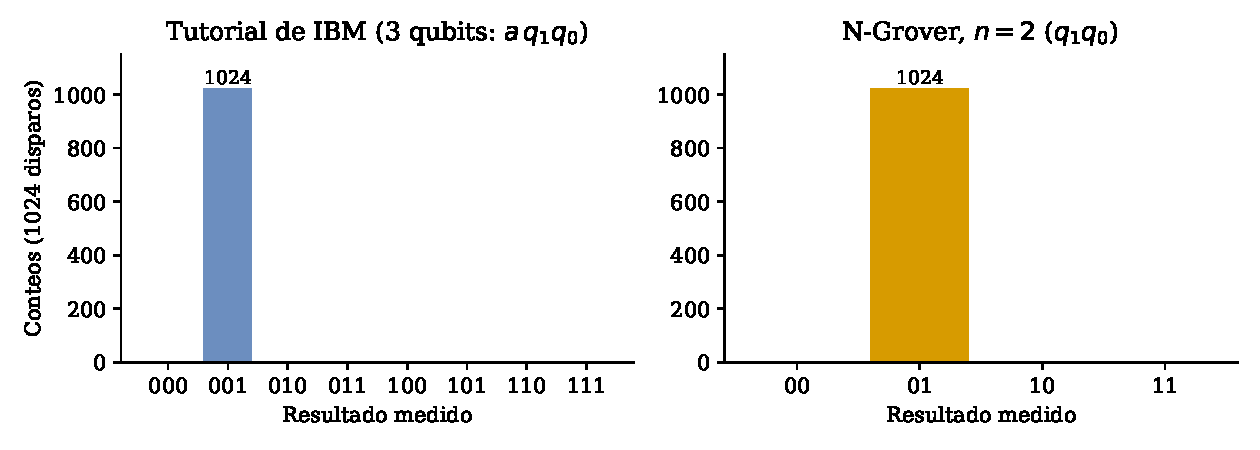
\includegraphics[width=0.95\textwidth]{../figuras/hist_tutorial_vs_ngrover.pdf}
\caption{Conteos con \texttt{AerSimulator} (1024 disparos). Izquierda: tutorial, resultado \texttt{001}
($a=0$, $q_1q_0=01$). Derecha: N-Grover, resultado \texttt{01}.}
\label{fig:hist}
\end{figure}

\subsection{Recursos}

\begin{table}[H]
\centering
\small
\begin{tabular}{@{}lcccc@{}}
\toprule
Circuito & Qubits & Profundidad & Compuertas (sin barreras ni medición) & Oracle en base $\{CX,R_z,\sqrt X\}$\\
\midrule
Tutorial & 3 & 15 & 10 $H$, 8 $X$, 1 $CCX$, 1 $CX$ & 6 $CX$\\
N-Grover & 2 & 14 & 10 $H$, 6 $X$, 2 $CX$ & 1 $CX$\\
\bottomrule
\end{tabular}
\caption{Tamaño de los circuitos antes de transpilar y costo del oracle al descomponerlo en compuertas nativas.}
\label{tab:recursos}
\end{table}

N-Grover usa un qubit menos, menos compuertas y ninguna Toffoli. La Toffoli no es nativa en hardware real y
se descompone en 6 CNOT, mientras que el oracle de N-Grover para $n=2$ usa una sola CNOT. Un detalle: al
transpilar para \texttt{AerSimulator}, N-Grover queda con profundidad~12 y el tutorial con~9, porque N-Grover
pone barreras dentro del difusor y el transpilador no puede fusionar compuertas a través de una barrera.
Esa diferencia es de presentación y desaparece si se quitan las barreras.

%==================================================================
\section{Comparación con el análisis manual (actividad 1)}

\subsection{Etapa por etapa}

En la actividad~1 se calcularon a mano los estados del circuito del tutorial~\cite{parte1,pasoapaso}.
Los estados de los datos (el auxiliar es un factor $\ket-$ separado) se comparan en la tabla~\ref{tab:manual}
con los que da el \texttt{Statevector} de N-Grover al final de cada bloque.

\begin{table}[H]
\centering
\small
\renewcommand{\arraystretch}{1.6}
\begin{tabularx}{\textwidth}{@{}>{\raggedright}p{2.2cm}>{\raggedright}p{4.6cm}>{\centering}p{2.6cm}>{\centering}p{2.6cm}>{\centering\arraybackslash}X@{}}
\toprule
Etapa & Manual (actividad 1) & Manual (vector) & N-Grover (simulado) & ¿Coincide?\\
\midrule
Inicialización ($\psi_2$) & $\frac12\big(\ket{00}+\ket{01}+\ket{10}+\ket{11}\big)$ & $\frac12(1,1,1,1)$ & $(0.5,0.5,0.5,0.5)$ & Sí\\
Oracle ($\psi_5$) & $\frac12\big(\ket{00}-\ket{01}+\ket{10}+\ket{11}\big)$ & $\frac12(1,-1,1,1)$ & $(0.5,-0.5,0.5,0.5)$ & Sí\\
Difusor ($\psi_{12}$) & $-\ket{01}$ & $(0,-1,0,0)$ & $(0,-1,0,0)$ & Sí\\
\bottomrule
\end{tabularx}
\caption{Estados de los datos $\ket{q_1q_0}$ al final de cada etapa. La numeración $\psi_k$ es la del documento paso a paso de la actividad~1.}
\label{tab:manual}
\end{table}

Los tres estados coinciden exactamente, incluido el signo $-1$ final. Además, en cada etapa el estado del
tutorial es $\ket-\otimes(\text{estado de N-Grover})$: el auxiliar no se entrelaza con los datos y solo sirve
para producir el cambio de fase.

\subsection{Dentro del oracle}

Aquí los circuitos usan compuertas distintas, así que solo coinciden al inicio y al final de la etapa. En
N-Grover los estados intermedios son:

\begin{table}[H]
\centering
\small
\begin{tabular}{@{}ll@{}}
\toprule
Después de & Estado de los datos\\
\midrule
Entrada & $\tfrac12\big(\ket{00}+\ket{01}+\ket{10}+\ket{11}\big)$\\
$X_1$ & $\tfrac12\big(\ket{00}+\ket{01}+\ket{10}+\ket{11}\big)$ \quad (no cambia: $X\ket+=\ket+$)\\
$H_1$ & $\tfrac{1}{\sqrt2}\big(\ket{00}+\ket{01}\big)$\\
$CX_{0\to1}$ & $\tfrac{1}{\sqrt2}\big(\ket{00}+\ket{11}\big)$\\
$H_1$ & $\tfrac12\big(\ket{00}+\ket{01}+\ket{10}-\ket{11}\big)$ \quad (la $CZ$ marcó $\ket{11}$)\\
$X_1$ & $\tfrac12\big(\ket{00}-\ket{01}+\ket{10}+\ket{11}\big)$ \quad (el signo pasa a $\ket{01}$)\\
\bottomrule
\end{tabular}
\caption{Estados intermedios del oracle de N-Grover.}
\end{table}

El primer paso coincide con el paso~3 de la actividad~1 ($X\ket+=\ket+$). Los pasos con $H_1$ y la CNOT generan
estados que no existen en el tutorial, porque allí el signo llega desde el auxiliar. El estado de salida es el
mismo $\psi_5$ del cálculo manual.

\subsection{Dentro del difusor}

El difusor de N-Grover es la misma secuencia del tutorial, así que sus siete capas deben reproducir los pasos
6 a 12 del documento paso a paso. Así ocurre:

\begin{table}[H]
\centering
\small
\begin{tabular}{@{}lll@{}}
\toprule
Paso & Capa & Estado manual $=$ simulado\\
\midrule
$\psi_6$ & $H$ en $q_1,q_0$ & $\tfrac12(1,1,-1,1)$\\
$\psi_7$ & $X$ en $q_1,q_0$ & $\tfrac12(1,-1,1,1)$\\
$\psi_8$ & $H$ en $q_1$ & $\tfrac1{\sqrt2}(1,0,0,-1)$\\
$\psi_9$ & $CX_{0\to1}$ & $\tfrac1{\sqrt2}(1,-1,0,0)$\\
$\psi_{10}$ & $H$ en $q_1$ & $\tfrac12(1,-1,1,-1)$\\
$\psi_{11}$ & $X$ en $q_1,q_0$ & $\tfrac12(-1,1,-1,1)$\\
$\psi_{12}$ & $H$ en $q_1,q_0$ & $(0,-1,0,0)$\\
\bottomrule
\end{tabular}
\caption{Capas del difusor: los siete estados simulados coinciden con los calculados a mano.}
\end{table}

Se ven los mismos efectos de la actividad~1: en $\psi_8$ los datos quedan en el estado de Bell
$\tfrac1{\sqrt2}(\ket{00}-\ket{11})$; los pasos 8--10 ($H$--CNOT--$H$) cambian solo el signo de $\ket{11}$; y en $\psi_{12}$
toda la amplitud está en $\ket{01}$.

\subsection{Inversión respecto a la media}

Después del oracle las amplitudes son $(\tfrac12,-\tfrac12,\tfrac12,\tfrac12)$, con media $\langle a\rangle=\tfrac14$. La reflexión
$a_x\mapsto 2\langle a\rangle-a_x$ da $(0,1,0,0)$. El difusor del circuito, $D_c=-(2\ketbra ss-I)$, da el negativo,
$(0,-1,0,0)$, que es justamente lo que muestran tanto el cálculo manual como el \texttt{Statevector}.

\subsection{Probabilidades}

\begin{table}[H]
\centering
\small
\begin{tabular}{@{}lccc@{}}
\toprule
Estado & Manual & \texttt{Statevector} & Muestreo (1024 disparos)\\
\midrule
$\ket{00}$ & 0 & 0 & 0\\
$\ket{01}$ & 1 & 1 & 1\\
$\ket{10}$ & 0 & 0 & 0\\
$\ket{11}$ & 0 & 0 & 0\\
\bottomrule
\end{tabular}
\caption{Probabilidad de cada resultado al final del algoritmo.}
\end{table}

Las tres columnas coinciden. El muestreo da exactamente~1 porque la probabilidad teórica de $\ket{01}$ es~1 y no hay
variación estadística. El signo $-1$ se ve en el \texttt{Statevector} y en el cálculo manual, pero desaparece al medir
porque $|-1|^2=1$.

%==================================================================
\section{Número de iteraciones para 2 qubits}
\label{sec:iter}

Con $N=4$ y un estado marcado, $\sin\theta=1/\sqrt N=\tfrac12$, así que $\theta=30^\circ$. Después de $k$ iteraciones la
amplitud del estado marcado es $\sin\big((2k+1)\theta\big)$. La fórmula $k\approx\frac\pi4\sqrt{N}=\frac\pi4\cdot2\approx1.57$
se redondea a $k=1$.

\begin{table}[H]
\centering
\small
\begin{tabular}{@{}cccc@{}}
\toprule
$k$ & $(2k+1)\theta$ & $P(\ket{01})$ teórica & $P(\ket{01})$ simulada\\
\midrule
0 & $30^\circ$ & 0.25 & 0.25\\
1 & $90^\circ$ & 1 & 1\\
2 & $150^\circ$ & 0.25 & 0.25\\
3 & $210^\circ$ & 0.25 & 0.25\\
\bottomrule
\end{tabular}
\caption{Probabilidad de éxito según el número de iteraciones para $n=2$.}
\end{table}

Con una iteración el estado llega exactamente a $\ket{01}$. Una segunda iteración lo pasa de largo y la probabilidad
vuelve a $\tfrac14$: los cuatro resultados quedan equiprobables (figura~\ref{fig:iter}). Por eso, para 2 qubits se usa
una iteración, como en el tutorial; las dos iteraciones del notebook original corresponden a $n=3$.

\begin{figure}[H]
\centering
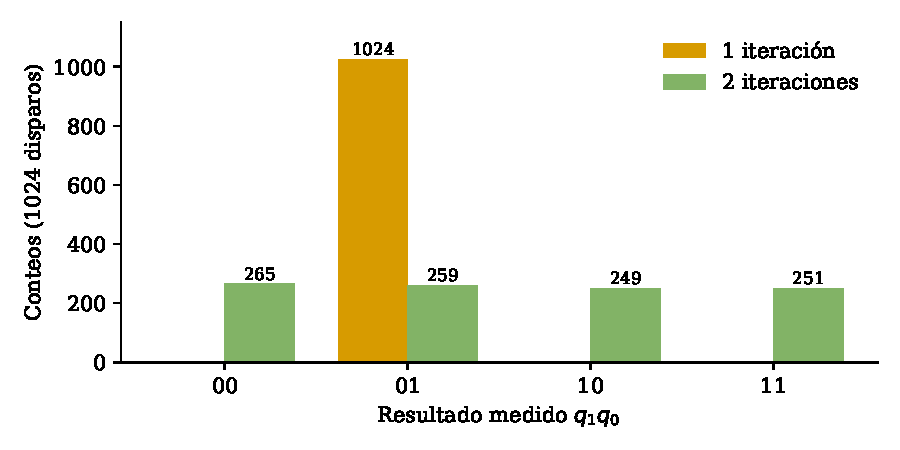
\includegraphics[width=0.62\textwidth]{../figuras/hist_iteraciones.pdf}
\caption{N-Grover con 2 qubits: una iteración da siempre \texttt{01}; dos iteraciones reparten los disparos de forma
aproximadamente uniforme (variación estadística del muestreo).}
\label{fig:iter}
\end{figure}

%==================================================================
\section{Conclusiones}

\begin{itemize}
\item \textbf{N-Grover generaliza el tutorial sin cambiar el algoritmo.} Para $n=2$ y \texttt{MarkState = '01'}, su oracle es
$I-2\ketbra{01}{01}$ y su difusor es $I-2\ketbra ss$: las mismas matrices que el tutorial aplica sobre los datos y las
mismas que se obtuvieron a mano en la actividad~1.
\item \textbf{La diferencia está en cómo se marca el estado.} El tutorial usa un auxiliar en $\ket-$ y una Toffoli
(retroceso de fase) con el estado fijo en el código. N-Grover usa una $Z$ multicontrolada ($H\cdot\mathrm{MCX}\cdot H$)
rodeada de $X$ en los qubits con dígito~0. No necesita auxiliar ni limpieza, usa menos compuertas y sirve para cualquier
estado y cualquier $n$.
\item \textbf{Los resultados coinciden.} El tutorial da \texttt{\{'001': 1024\}} y N-Grover \texttt{\{'01': 1024\}}: el mismo
resultado sobre $q_1q_0=01$; el \texttt{0} extra del tutorial es el auxiliar limpio. Los vectores de estado cumplen
$\ket{\Psi_{\text{tutorial}}}=\ket0\otimes\ket{\psi_{\text{N-Grover}}}=-\ket{001}$.
\item \textbf{El análisis manual queda confirmado.} Los estados simulados de inicialización, oracle y difusor, y las siete
capas internas del difusor, coinciden con los calculados a mano, incluido el signo $-1$ final (fase global, sin efecto
en la medición).
\item \textbf{Para 2 qubits hay que ajustar las iteraciones.} La celda~7 del original tiene el estado \texttt{'011'} fijo y
falla con $n=2$; además, con dos iteraciones la probabilidad de éxito baja de~1 a~$\tfrac14$. Lo correcto es una iteración.
\end{itemize}

\paragraph{Entorno.} Notebooks y figuras ejecutados con Qiskit 2.5.2, Qiskit Aer 0.18.2, Qiskit IBM Runtime 0.51.0 y Python 3.13.

%==================================================================
\begin{thebibliography}{9}

\bibitem{ibm}
A.~Matsuo, ``Quantum algorithms: Grover Search and applications'', curso \emph{Utility-scale quantum
computing}, IBM Quantum Learning, 2024. Secciones~2.1 y~2.2.
\url{https://quantum.cloud.ibm.com/learning/en/courses/utility-scale-quantum-computing/grovers-algorithm}

\bibitem{ngrover}
Notebook del curso \texttt{N-Grover\_AnyMark\_2026.ipynb}.
\url{https://github.com/gpatigno/QC_POSGRADO_2026/blob/main/LAB/PR3/N-Grover_AnyMark_2026.ipynb}

\bibitem{parte1}
J.~D. Zapata Londoño, Práctica~3, actividad~1: análisis matemático a mano del circuito de Grover de 2 qubits (publicado por separado).

\bibitem{pasoapaso}
J.~D. Zapata Londoño, Práctica~3, actividad~1: desarrollo paso a paso, estados $\psi_0$ a $\psi_{14}$ (publicado por separado).

\bibitem{grover}
L.~K. Grover, ``A fast quantum mechanical algorithm for database search'', en \emph{Proceedings of
the 28th Annual ACM Symposium on Theory of Computing (STOC '96)}, pp.~212--219, 1996.
\url{https://doi.org/10.1145/237814.237866}

\bibitem{enunciado}
Enunciado de la Práctica de Laboratorio No.~3: \texttt{Practica3\_Grover.md}, actividad~2.

\end{thebibliography}

\end{document}
